\documentclass[10pt,a4paper,openright]{article}
\usepackage{amsfonts}
\usepackage{float}
\usepackage[utf8]{inputenc}
\usepackage[T1]{fontenc}
\usepackage{graphicx}
\usepackage{amsmath,amssymb,verbatim}
\textheight=240mm
\textwidth=170mm
\topmargin=-15mm
\oddsidemargin=-6mm
\evensidemargin=\oddsidemargin
\newcommand\tab[1][1cm]{\hspace*{#1}}
\usepackage{hyperref}
\newcommand{\norm}[1]{\left\lVert#1\right\rVert}

\begin{document}
	\begin{flushleft}
		\large Name: Matouš Dzivjak\\
		\large Date: 9.11.2018\\
	\end{flushleft}
\begin{center}
	\huge PCA
\end{center}
\section{Zadání}
\begin{verbatim}
https://cw.fel.cvut.cz/wiki/courses/b33opt/cviceni/domaci_ulohy/kruznice/start
\end{verbatim}


\section{Řešení}

Ze zadání máme:
\begin{center}
$f(x) = \sum_{i=1}^{m}dist(x_i,a_i)^2$\\
\vspace{5mm}
$dist(x,a) = \sqrt{(a_0 - x_0)^2 + (a_1 - x_1)^2} - r$
\end{center}

\subsection{}
Mějme několik bodů $a_1,...,a_m$ v obecné konfiguraci.
Je funkce $f$ všude diferencovatelná? 
Má jedno nebo více lokálních minim?

Funkce není spojite diferencovatelná protože v bodě $a_0 = x_0, a_1 = x_1$ nemá derivaci.
Funkce má nekonečně mnoho lokálních minim. Např. pro jeden jediný bod
bude funkce nabývat minimam v jakémkoliv bodě, pokud za poloměr dosadíme vzdálenost bodu
od středu kružnice.

\subsection{}
Diskutujte, jaký algoritmus je vhodný na minimalizaci funkce $f(x)$ a proč.
Je možné, aby Gaussův-Newtonův algoritmus na naší úloze divergoval?

Gauss-Newtonova metoda konverguje pomaleji než ostatní metody.
Výhodou je, že u ní není nutné počítat druhé derivace. 
Levenberg-Marquardtova metoda je kombinací Gauss-Newtonovo a gradientní
metody - konverguje rychleji v okolí optima a zároveň zaručuje dostatečnou
spolehlivost i ve větší vzdálenosti od optima. U Levenberg-Marquardtovi metody
se také nestává, že by algoritmus nezkonvergoval, což se o Gauss-Newtonovo metodě
říci nedá.

\subsection{}
Může se zdát, že algoritmy na nelineární nejmenší čtverce bez omezení nejde použít, 
protože máme omezení $r \le 0$. Vadí to? 
Co se stane, budeme-li toto omezení ignorovat? 
Můžou algoritmy konvergovat k řešení se záporným $r$?

V hodně specifických případech by taková možnost nejspíše mohla nastat. Nicméně 
záporne $r$ by způsobilo nárůst criterionu (součet čtverců vzdáleností bodů od kružnice),
protože zatím co pro kladná $r$ se $r$ odčítá pro záporná by se jeho velikost přičítala.
Tedy ke konvergenci k zápornému číslu by dojít nemělo, což je důvod, proč jsem
ve své implementaci tuto možnost neošetřoval a při testování nenastal nikdy problém.

\subsection{}
Najděte nějakou množinu $m \le 3$ bodů $\{a_1,a_2,...,a_m\}$
a takovou dvojici počátečních parametrů kružnice $x^{(1)}_0$ a $x^{(2)}_0$, 
aby algoritmus inicializovaný těmito parametry skončil v různých lokálních minimech.

Za množinu bodů zvolíme: $\{(0,3),(1,0)\}$ pak pro $x^{(1)}_0 = (1, 1, 1)$ dostáváme kružnici, kde každý
bod leží na opačné straně kružnice, střed kružnice je na těžišti těchto dvou bodů a
poloměr odpovídá jejich vzdálenosti od středu kružnice, zatím co pro $x^{(2)}_0 = (20, 20, 30)$
dostáváme po konvergenci kružnici, kde oba body leží blízko sebe na kružnici a kružnice má
velký poloměr

\begin{center}
    \begin{tabular}{| l | l | l |}
    \hline
    body a kružnice $x^{(n)}_0$ & body a stav dokonvergovaný z $x^{(n)}_0$ & graf f\_history pro $x^{(n)}_0$ \\ \hline
    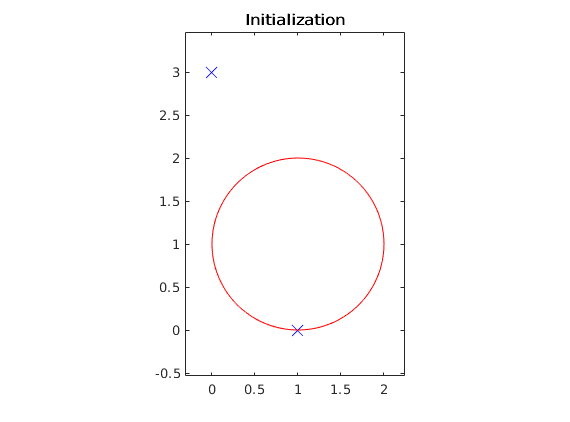
\includegraphics[scale=0.3]{conv1_init.png} & \includegraphics[scale=0.3]{conv1.png} & 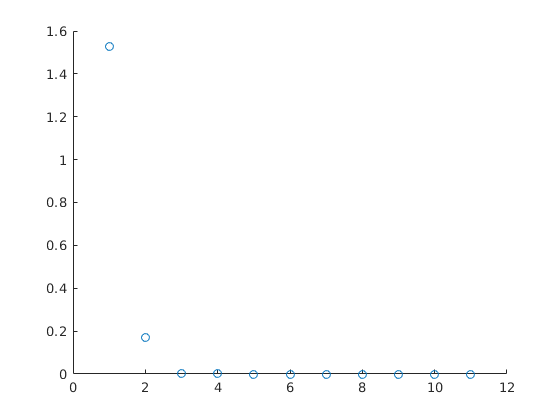
\includegraphics[scale=0.3]{conv1_history.png}\\ \hline
    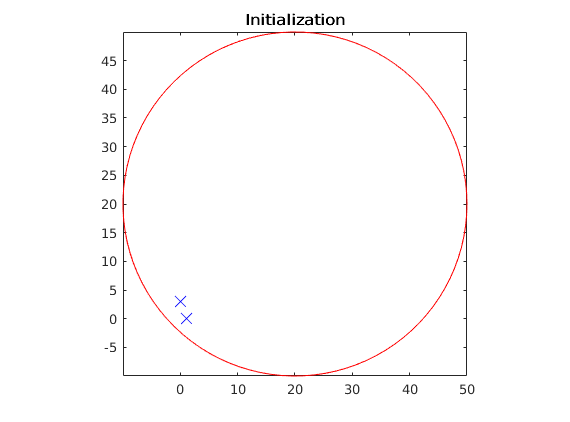
\includegraphics[scale=0.3]{conv2_init.png} & 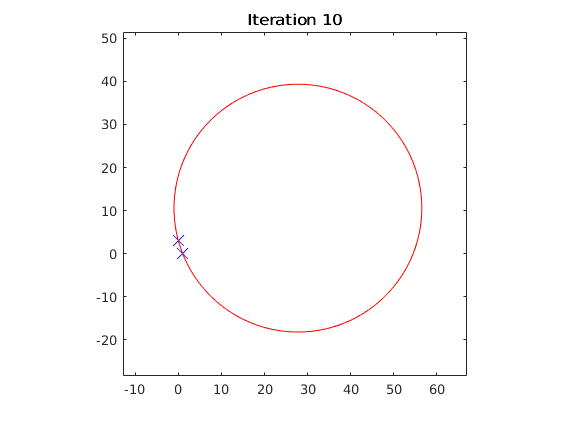
\includegraphics[scale=0.3]{conv2_end.png} & 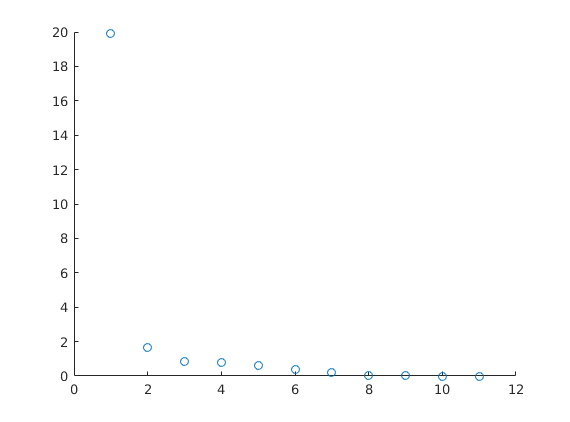
\includegraphics[scale=0.3]{conv2_history.png}\\ \hline
    \end{tabular}
\end{center}

\end{document}